
\section{State dependent discontinuity problem}
In this section, we consider the state-dependent discontinuity problem. We start by noting that this problem cannot be solved with the form of discontinuity handling used in the previous problem since we do not know when the discontinuity arises. Also, this problem will be more challenging than the time-dependent discontinuity problem as the parameter $\beta$ will be changed more than once as we attempt to model the periods of imposition of Covid-19 measures followed by periods where these measures are removed. 

As in Section $\ref{section:time_problem}$, changes in the modelling parameter $\beta$ introduce discontinuities in the function $f(t, y(t))$ and thus some solvers will ``thrash" when trying to solve the problem (as described in Section $\ref{subsection:effect_of_discontinuity}$). We will show that the presence of several discontinuities makes the problem challenging enough that all the ODE solvers we consider, even at very sharp tolerances, will not be able to solve the problem with reasonable accuracy.

The problem uses the state variable, E(t), which is the number of Exposed people, to determine when to change the parameter $\beta$. When the number of exposed people is greater than 25000, measures will be introduced and thus $\beta$ will change from 0.9 to 0.005. When the number of exposed people drops to 10000, the measures will be relaxed and $\beta$ is set to 0.9. We run this model over a longer time period toggling the parameter $\beta$ back and forth to model the periods of alternating the imposition and relaxing of the measures. This scenario corresponds to the case of an unvaccinated population where the only means of controlling the spread of the virus is through measures such as social isolation, masking, etc. The ability of the virus to infect people is not diminished as time progresses, and when measures to stop the spread of the virus are removed, the infection rate of the virus returns to its original value. More sophisticated models could be introduced by considering the $\beta$ parameter as a function of time. The numerical challenges would be similar.

We start with a simple treatment of the problem with if-statements applied inside the function that defines the right-hand side of the ODE system. We proceed to show how this form of the problem cannot be solved with reasonable accuracy, even at sharp tolerances. Finally, we will introduce an approach to efficiently and accurately solve the problem using event detection to handle the discontinuities.

\subsection{Simple treatment of Covid-19 state dependent discontinuity model}
\label{subsection:naive_state_problem}
A simple treatment of this problem is to use global variables for tracking when measures are implemented and relaxed and to toggle these global variables as we reach the required thresholds. Global variables are needed because we need to know if the number of exposed people is going up or down to know whether we need to check for the maximum or the minimum threshold. We then have an if-statement that will choose the value of parameter $\beta$ based on whether measures are being implemented or not. The pseudo-code for this algorithm is as follows:

\begin{minipage}{\linewidth}
\begin{lstlisting}[language=Python]
measures_implemented = False
direction = "up"

function model_with_if(_, y):
    // ...
    global measures_implemented, direction
    if (direction == "up"):
        if (E > 25000):
            measures_implemented = True
            direction = "down"
    else:
        if (E < 10000):
            measures_implemented = False
            direction = "up"

    if measures_implemented:
        beta = 0.005 
    else:
        beta = 0.9
    // ...
    return (dSdt, dEdt, dIdt, dRdt)
\end{lstlisting}
\end{minipage}

\subsubsection{Simple solution of the state dependent discontinuity model in R}
\begin{figure}[H]
\centering
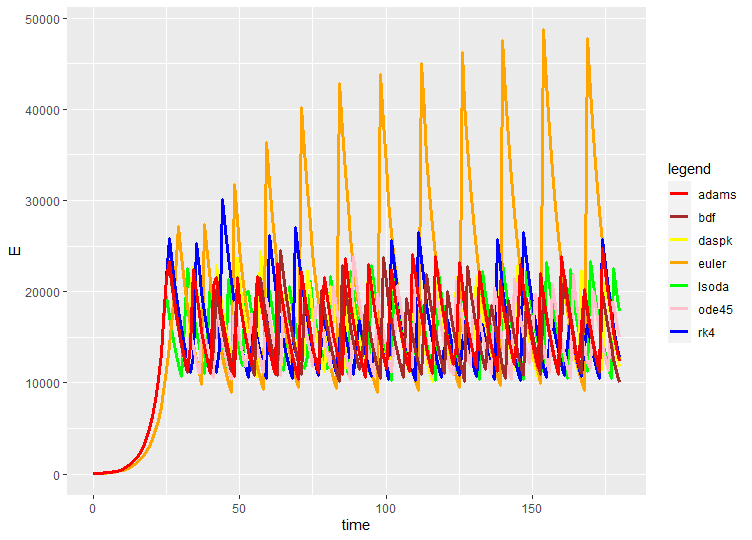
\includegraphics[width=0.7\linewidth]{./figures/state_discontinuity_R}
\caption{Solutions to the state dependent discontinuity model in R, based on the simple approach.}
\label{fig:state_discontinuity_R}
\end{figure}
In Figure $\ref{fig:state_discontinuity_R}$, we show the results from the use of a number of solvers in R based on the simple implementation described above using default tolerances. Figure $\ref{fig:state_discontinuity_R}$ shows how difficult this problem is with a simple treatment. We note that none of the solutions are aligned and that none of the solvers get a reasonably accurate solution (described in Section $\ref{subsection:state_with_event_detection}$) as none of the computed solutions cleanly oscillate between 10000 and 25000 with clear peaks and troughs.

We note that none of the solvers, even the error-controlled ones, issued a warning about the integration and thus users may be tempted to think that the solver has solved the problem to within reasonable accuracy. Having no warning also tells us that the error estimation and error control algorithms employed by all the solvers did not detect anything abnormal; the solvers return with an indication that the provided solutions are accurate to within the requested tolerance.

As we are modeling E(t), we expect that each graph should go from 25000 to 10000 and back to 25000 repeatedly but none of these graphs do so in the required pattern. We would also expect the solvers with error control to repeatedly reduce the step-size to satisfy the tolerance and compute solutions that align with each other but Figure $\ref{fig:state_discontinuity_R}$ shows that this is not the case.

We also note that the result for `euler' is especially poor as it reaches a maximum of 40000. This is again as expected as `euler' has no error control; `rk4', the other fixed step-size method, is also performing poorly; we see the solution it computes reach approximately 30000 in its third peak. This is happening even though the space between the output points is as small as it was when we were investigating the time-dependent discontinuity problem. Because of this, we will not run any spacing of output points experiments in this section. The step-size for these fixed-step solvers is not small enough and further step-size reductions are needed.

Another important fact to note is how poorly `Radau', as shown in Figure $\ref{fig:state_discontinuity_radau_R}$, performs. This is not a problem with the R programming environment as similar results will be seen in Python in the next section and in the Fortran code in Section $\ref{section:fortran_inaccuracies}$. The solution grows exponentially even after the parameter $\beta$ is switched to 0.005, which should force the solution to begin a decay. We perform an analysis with the Fortran code later in this report to show that $\beta$ is indeed 0.005 while this exponential growth is happening. 

\begin{figure}[h]
\centering
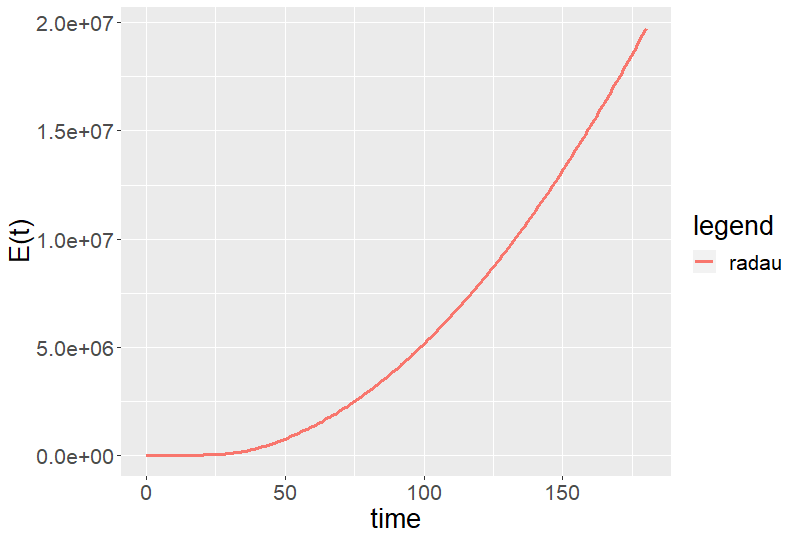
\includegraphics[width=0.7\linewidth]{./figures/state_discontinuity_radau_R}
\caption{Solution by `Radau' for the state dependent discontinuity model in R, based on the simple approach.}
\label{fig:state_discontinuity_radau_R}
\end{figure}

We next proceed to show that sharp tolerances are not enough to solve this problem as was the case for the time-dependent discontinuity problem. We repeat the experiment at the sharpest tolerance that could be used prior to some of the solvers failing. This was at $10^{-13}$ in the R environment. We set both the absolute and relative tolerance to that value and show the results in Figure $\ref{fig:state_discontinuity_sharp_R}$.

\begin{figure}[H]
\centering
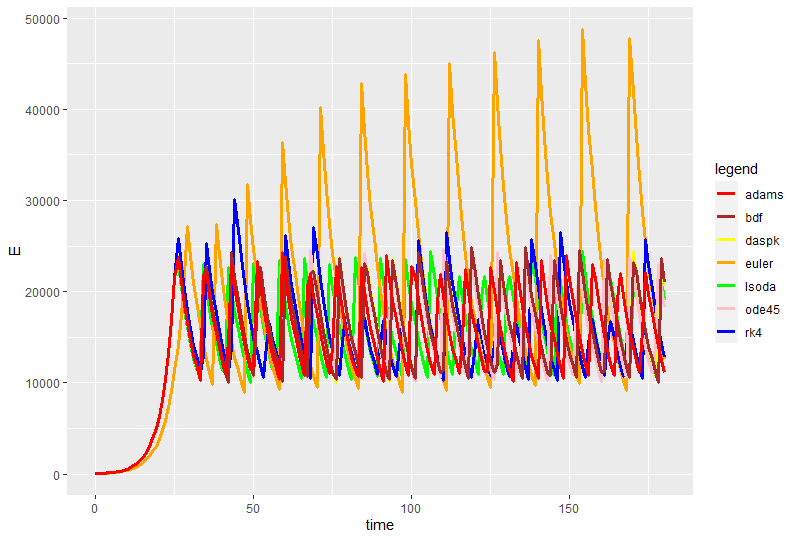
\includegraphics[width=0.7\linewidth]{./figures/state_discontinuity_sharp_R}
\caption{Solutions to the state dependent discontinuity model in R with a sharp tolerance, using the simple approach.}
\label{fig:state_discontinuity_sharp_R}
\end{figure}

We can see from Figure $\ref{fig:state_discontinuity_sharp_R}$ that the situation has only marginally improved. None of the solvers give solutions that are in agreement with each other and none of the solutions cleanly oscillate between 10000 and 25000. We note that the error-controlled solvers are following the correct pattern and that until about time 20-30, some of them give solutions that are in agreement, showing that sharp tolerance error-control can step over one state-dependent discontinuity. (See the comparison against the final solution in Section $\ref{subsubsection:state_solution_comparison}$ to see that even this sharp tolerance solution is not accurate enough.)

The fixed step-size method `euler' and `rk4' results are the same as in Figure $\ref{fig:state_discontinuity_R}$ since these codes do not employ a tolerance.

We can also point out that at such sharp tolerances `Radau' no longer computes solutions exhibiting the abnormal behavior we saw previously. From Figure $\ref{fig:state_discontinuity_radau_sharp_R}$, we can see that the solution computed by `Radau' oscillates approximately between 10000 and 25000. From supplementary experiments, we observe that `Radau' starts performing at a level that is comparable to the other solvers at a tolerance of $10^{-9}$ or sharper.

\begin{figure}[H]
\centering
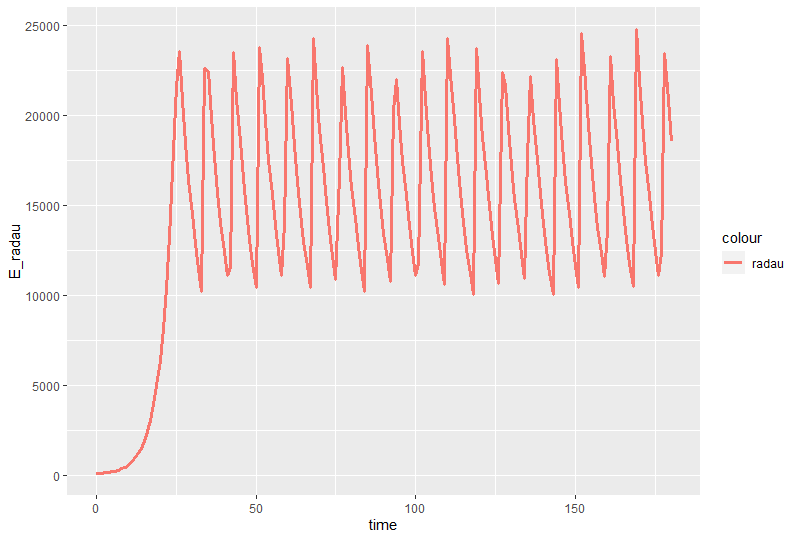
\includegraphics[width=0.7\linewidth]{./figures/state_discontinuity_sharp_radau_R}
\caption{Solution by `Radau' for the state dependent discontinuity model in R with a sharp tolerance, using the simple approach.}
\label{fig:state_discontinuity_radau_sharp_R}
\end{figure}

\subsubsection{Simple solution of the state dependent discontinuity model in Python}
\begin{figure}[H]
\centering
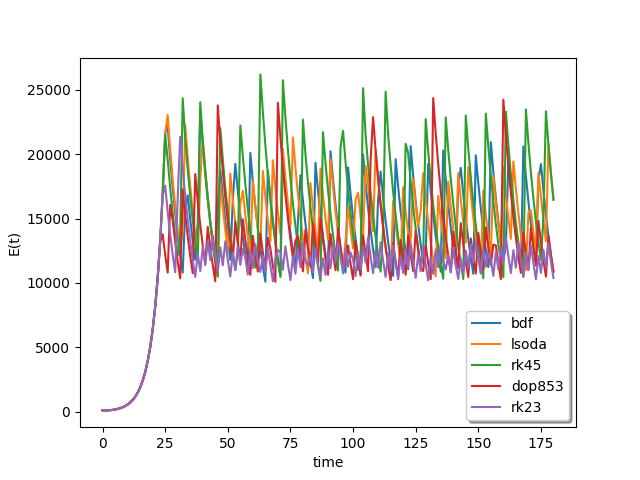
\includegraphics[width=0.7\linewidth]{./figures/state_discontinuity_py}
\caption{Solutions to the state dependent discontinuity model in Python, based on the simple approach.}
\label{fig:state_discontinuity_python}
\end{figure}
Figure $\ref{fig:state_discontinuity_python}$ shows what happens when the problem is solved using the simple implementation and default tolerances in Python. We can see that the results are similar to those obtained in R. This happens even though all solvers in Python have error control.

We note that all the solvers except `RK23' give solutions that at least oscillate between 10000 and 25000, though in completely dissimilar patterns. The solutions have peaks and troughs at different times. No warnings were given by the solvers.

The `RK23' solver, whose solution is shown in purple, computes a solution with a completely different pattern than the other solvers. It never reaches 25000 and only oscillates between around 10000 and 15000. 

Again, as shown in Figure $\ref{fig:state_discontinuity_radau_py}$, `Radau' computes a solution that has E(t) growing exponentially even though the parameter $\beta$ is eventually set to 0.005 which should give a solution with an exponential decay in the E(t) component as we see with all other solvers.

\begin{figure}[h]
\centering
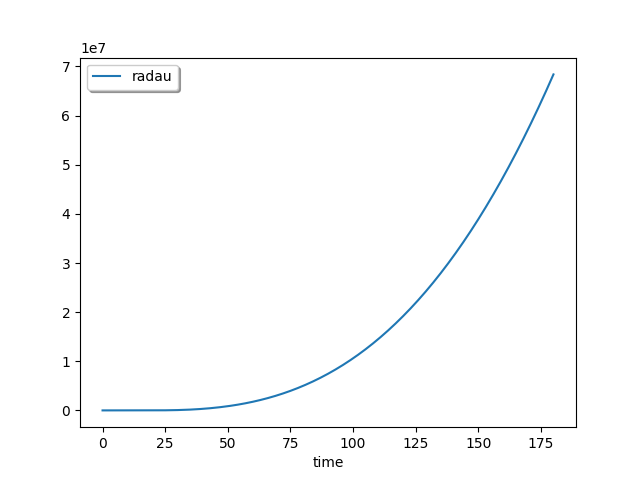
\includegraphics[width=0.7\linewidth]{./figures/state_discontinuity_radau_py}
\caption{Solution by `Radau' for the state dependent discontinuity model in Python, based on the simple approach.}
\label{fig:state_discontinuity_radau_py}
\end{figure}

We then used very sharp tolerances to solve the problem but, as is the case in the R environment, none of the solvers obtained a reasonably accurate solution. The highest tolerance we could use in Python without any one method failing was $10^{-12}$. Both the absolute and relative tolerances were set to this value and Figure $\ref{fig:state_discontinuity_sharp_python}$ shows the results from this sharp tolerance experiment.

\begin{figure}[H]
\centering
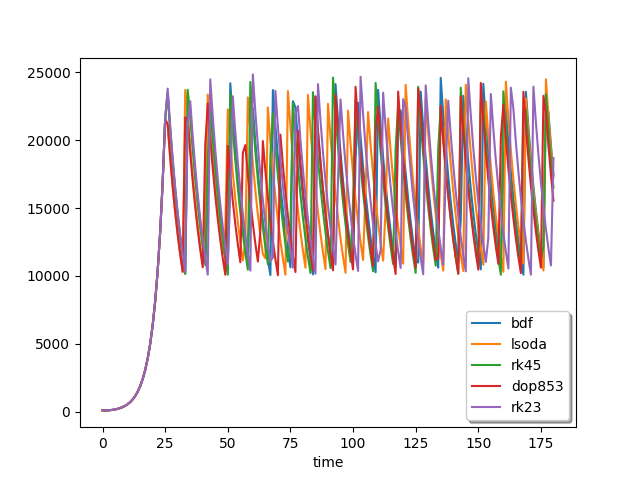
\includegraphics[width=0.7\linewidth]{./figures/state_discontinuity_sharp_py}
\caption{Solutions to the state dependent discontinuity model in Python with a sharp tolerance, using the simple approach.}
\label{fig:state_discontinuity_sharp_python}
\end{figure}

Figure $\ref{fig:state_discontinuity_sharp_python}$ shows that the results did improve. However, the solvers give solutions that are not in agreement. We note that none of the solvers are oscillating beyond 25000 as was the case with the fixed-step solvers in R. At sharp tolerances, the solutions are aligned for the first few discontinuities with only some blurring until about t=25 when the solvers give substantially different solutions. Though the pattern is correct, none of the solvers give solutions that are in agreement telling us that none were able to compute a reasonably accurate solution such as the one that we present in Section $\ref{subsection:state_with_event_detection}$. (See the comparison against the final solution in Section $\ref{subsubsection:state_solution_comparison}$ to see that even this sharp tolerance solution is not accurate enough.)

We note that `RK23' is now following the correct pattern in that it oscillates between 10000 and 25000 whereas it only reached 15000 at the default tolerance. 

\begin{figure}[H]
\centering
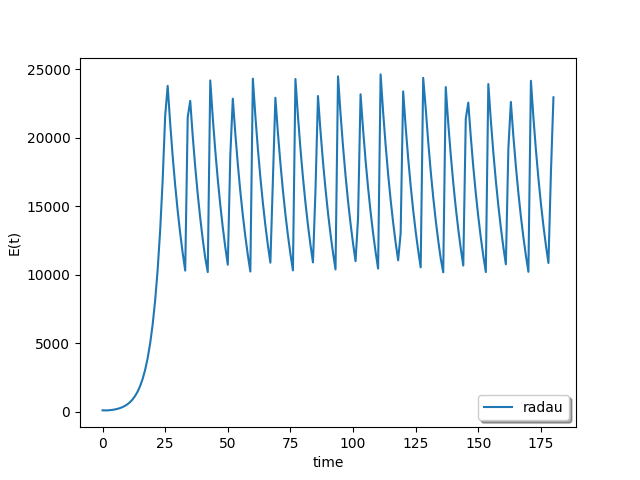
\includegraphics[width=0.7\linewidth]{./figures/state_discontinuity_sharp_radau_py}
\caption{Solution by `Radau' for the state dependent discontinuity model in Python with a sharp tolerance, using on the simple approach.}
\label{fig:state_discontinuity_sharp_radau_py}
\end{figure}

Again, as shown in Figure $\ref{fig:state_discontinuity_sharp_radau_py}$, the `Radau' solver begins to give reasonable solutions at these sharp tolerances; the solutions follows the pattern we are expecting but as we will show in Section $\ref{subsection:state_with_event_detection}$, they are still not sufficiently accurate solutions. The `Radau' solver starts performing reasonably well at around a tolerance of $10^{-10}$. We also note that the R and Python implementation of `Radau' are different. The `Radau' solver in Python is implemented in Python with the NumPy library whereas R uses the Fortran code. Thus we eliminate the possibility of a bug in the code as well as any problem stemming from the interface from R to Fortran or from Python to NumPy. The problem is simply in how the Radau algorithm interacts with this simple implementation of the state-dependent discontinuity. In our experiments with the Radau Fortran code, in Section $\ref{section:fortran_inaccuracies}$, the same behavior is observed.

\subsubsection{Simple solution of the state dependent discontinuity model in Scilab}
\begin{figure}[H]
\centering
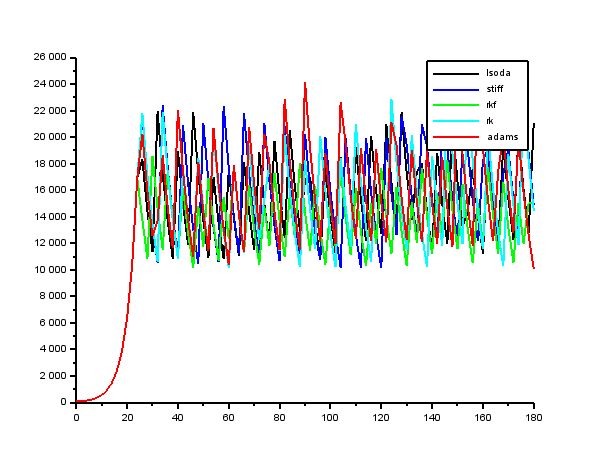
\includegraphics[width=0.7\linewidth]{./figures/state_discontinuity_scilab}
\caption{Solutions to the state dependent discontinuity model in Scilab, based on the simple approach.}
\label{fig:state_discontinuity_scilab}
\end{figure}

Figure $\ref{fig:state_discontinuity_scilab}$ shows the same issues that we saw before. None of the solvers give solutions that are aligned which prompts us to conclude that none of them are getting a reasonably accurate solution. All of the solvers in Scilab have error control and we can also see that their solutions all follow the correct pattern of oscillating approximately between 10000 and 25000. However, as we will discuss in Section $\ref{subsection:state_with_event_detection}$, none of the solutions are very accurate. We note that the spacing between output points is not important in this analysis as at the current spacing, even the solvers that depend on the spacing are getting inaccurate answers.

We then repeat the experiment at sharp tolerances. The Scilab `rkf' method does not allow the use of very sharp tolerance as it has a cap of 3000 derivative evaluations so it was omitted from this experiment. The sharpest tolerance we can use in Scilab before the other methods fail is $10^{-13}$; the results are shown in Figure $\ref{fig:state_discontinuity_sharp_scilab}$.

\begin{figure}[H]
\centering
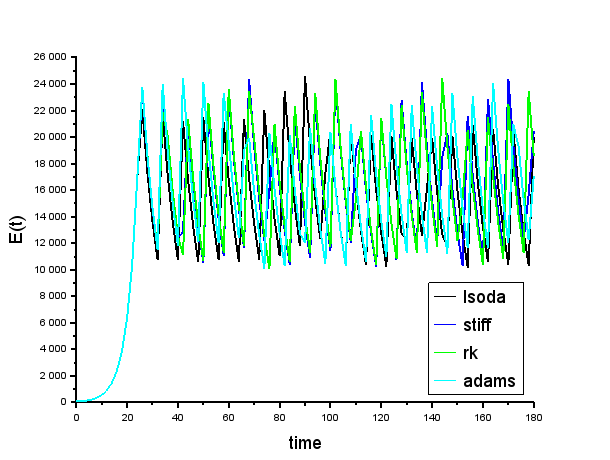
\includegraphics[width=0.7\linewidth]{./figures/state_discontinuity_sharp_sci}
\caption{Solutions to the state dependent discontinuity model in Scilab with a sharp tolerance, using the simple approach.}
\label{fig:state_discontinuity_sharp_scilab}
\end{figure}

Again, in Figure $\ref{fig:state_discontinuity_sharp_scilab}$ we can see that the use of sharp tolerances is not enough to force the solvers to compute reasonably accurate solutions. The solutions did improve as all the solvers follow the correct pattern but none oscillate between 10000 and 25000 with clear peaks and troughs at those values. For the time period between 0 to 30, the solutions all seem to show reasonable agreement but as we go further in time, all of the solutions diverge. We also note that none of the solvers compute solutions in reasonable agreement with the solution discussed in Section $\ref{subsection:state_with_event_detection}$. (See the comparison against the final solution in Section $\ref{subsubsection:state_solution_comparison}$ to see that even these sharp tolerance solutions are not accurate enough.)


\subsubsection{Simple solution of the state dependent discontinuity model in Matlab}
\begin{figure}[H]
\centering
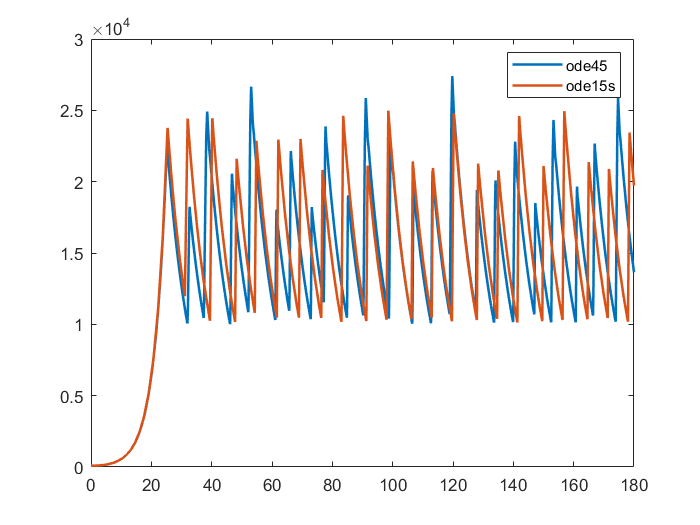
\includegraphics[width=0.7\linewidth]{./figures/state_discontinuity_matlab}
\caption{Solutions to the state dependent discontinuity model in Matlab, based on the simple approach.}
\label{fig:state_discontinuity_matlab}
\end{figure}
In Figure $\ref{fig:state_discontinuity_matlab}$. we see the same incorrect solutions in Matlab as we did in the previous environments as the solvers are run with the simple implementation at the default tolerances. The solvers do not even consistently reach 25000. We then use a sharper tolerance to see if the solutions are improved.

\begin{figure}[h]
\centering
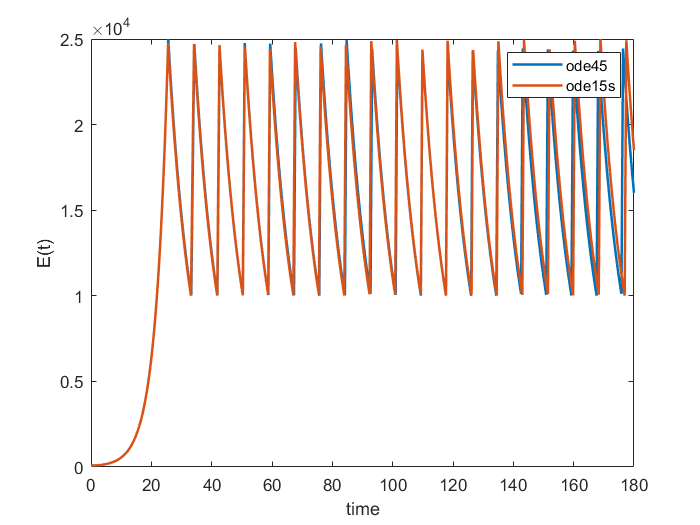
\includegraphics[width=0.7\linewidth]{./figures/state_discontinuity_sharp_matlab}
\caption{Solutions to the state dependent discontinuity model in Matlab with a sharp tolerance, using the simple approach.}
\label{fig:state_discontinuity_sharp_matlab}
\end{figure}

Figure $\ref{fig:state_discontinuity_sharp_matlab}$ shows the results of the experiment at sharp tolerances. We get surprisingly good solutions compared to the solutions in the previous environments. However, as we will see in Section $\ref{subsection:state_with_event_detection}$, these solutions are computed extremely inefficiently and they are not as accurate as the solution presented in Section $\ref{subsection:state_with_event_detection}$, especially for later time periods. (See the comparison against the final solution in Section $\ref{subsubsection:state_solution_comparison}$ to see that even these sharp tolerance solutions are not accurate enough.)


\subsubsection{State dependent discontinuity model - solution comparisons}
\label{subsubsection:state_solution_comparison}
In all the previous subsections, we have maintained that even the sharp tolerance solutions, though more in agreement, are not accurate. Here, we present a comparison between the solution obtained by LSODA in Python using the simple approach at the default tolerance and at the sharpest tolerance, alongside an accurate solution that we will present shortly which is obtained using event detection. We can see from Figure $\ref{fig:comparison_state_default_sharp_event}$ that the solutions from LSODA both at default and the sharp tolerance obtained using the simple approach do not agree with the more accurate solution. 

\begin{figure}[H]
\centering
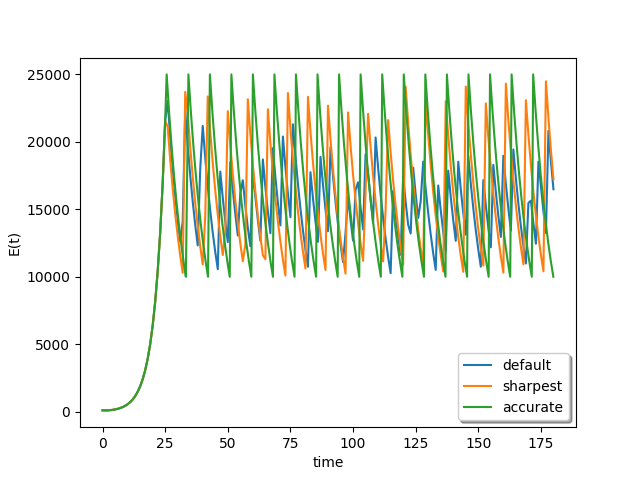
\includegraphics[width=0.7\linewidth]{./figures/comparison_state_default_sharp_event}
\caption{Solutions to the state dependent discontinuity model from LSODA based on the simple approach using the default tolerance and a sharp tolerance, alongside an accurate solution.}
\label{fig:comparison_state_default_sharp_event}
\end{figure}

\subsection{Why the solvers fail even with sharp tolerances}
\label{subsection:state_sharp_tol_failed}
In this section we discuss why sharp tolerances were not enough to force the solvers to accurately solve the problem in the simple way it is coded, i.e, using global variables and if-statements. 

Whenever there is a change in the value of $\beta$, the step where the discontinuity is first encountered will almost always be a failed step. As discussed in Section $\ref{subsection:effect_of_discontinuity}$, the step-size at a discontinuity will always have to be much smaller than the step-size on the continuous region to the left of the discontinuity. Thus the first encounter of a solver with any discontinuity will always be in the context of a failed step.

During this failed step, the value of E(t) will cross the threshold. The global variables will thus be toggled. But then, when the solver attempts to retake the step using a smaller step-size, to the left of the discontinuity, it will be using the wrong $\beta$ value. 

This observation is crucial as it allows us to conclude that once a failed step has occurred due to the solver encountering a discontinuity, the function evaluations made to the left of the discontinuity should be based on the previous $\beta$ value but they are in fact obtained using the new $\beta$ value. There is no trivial way to code this behavior in the ODE function, $f(t, y(t))$, since we do not know the time of the discontinuity. 

The problem, in summary, is that the solvers need to figure out how to step up to the discontinuity such that to the left of the discontinuity, the solver employs function evaluations that use the previous $\beta$, and then after the discontinuity, the solver employs function evaluations that use the new $\beta$ value. This cannot be coded in a straightforward way using the interfaces available in the programming environments.

In the next few sections, we will present a better approach for treating problems with state-dependent discontinuities that will allow us to get reasonably accurate solutions in an efficient manner.

\subsection{Event detection}
\label{subsection:intro_event_detection}
For the time-dependent discontinuity problem, we saw that if we used error-controlled software, then the solvers can accurately work through one discontinuity at sufficiently high tolerances. We also showed that this was not the most efficient way to solve the problem. For the state-dependent discontinuity problem, we showed in the previous section that the solvers, using even sharp tolerances, are not be able to solve this problem with much accuracy. Because we do not know when the discontinuities occur, we cannot use the discontinuity handling technique, involving a cold restart, that we used to solve the time-dependent discontinuity problem. However, the idea that we developed in Section $\ref{subsection:time_disc_handling}$ about integrating continuous sub-problems separately and combining them into a final solution can be applied here. 

To integrate continuous sub-problems, we need a way to detect that a threshold has been met, and then as soon as we reach such a point, we can perform a cold start. This will make the solver integrate the problem one continuous subinterval at a time. In this section, we will explain the capability of modern solvers to detect events and we will show how to encode the E(t) thresholds (either E(t)=25000 or E(t)=10000) as events so that the times at which they occur can be determined. We can then perform a cold start at these times.

To perform event detection, an ODE solver requires two functions from the user: the usual ODE right-hand side function, $f(t, y(t))$ and another function, the root function (commonly denoted by $g(t, y(t))$), that defines the events.

The root function is a function that, given the value of the solution $y(t)$ at time $t$ to the ODE at the current step will return a number. The event function, $g(t, y(t))$, is said to have a root whenever the value of the root function is zero. The key idea is that each event must be written so that it occurs at the root of a root function.

The solver calls the root function at the end of each successful step that it takes and will record its value. It will then compare the value of the root function with the corresponding value from the previous step to see if there has been a change of sign. If the value of the root-function has changed sign, the solver will then run a root-finding algorithm on that step to find the point where the root-function equals zero. Most solvers will then return, allowing us to perform a cold start.

Using event detection thus entails defining a function that takes the value of the ODE solution at the current point and returns a real number which is zero whenever there is an event. For example, if we want to detect when y is 100, it is sufficient to define (y - 100) to be the root function. In the next section, we will elaborate on how to use event detection to accurately and efficiently solve the state-dependent discontinuity problem.

We also mention that many modern solvers have event detection built-in. Thus users should be able to use event-detection solvers from their preferred programming environments without any additional software, being required.

\subsection{Solving the state dependent discontinuity model using event detection}
\label{subsection:state_with_event_detection}
As mentioned earlier, each toggling between the values of the parameter $\beta$ introduces a discontinuity. As none of the provided solvers are designed to solve discontinuous problems, we get the erroneous solutions reported in $\ref{subsection:naive_state_problem}$. We have seen that although sharp tolerances do result in somewhat better solutions being computed, none of the solvers were able to obtain a sufficiently accurate solution. The use of such sharp tolerances leads to inefficiencies as well. We will now present an approach using event detection that is both accurate and efficient.

The idea is to use the thresholds that we have defined in our model to define events and integrate up to the time at which each threshold is reached using the event detection capability of the solver. We can then cold start from there and repeat the process with another right-hand side function corresponding to the new $\beta$ value and with a different root function that encodes the next threshold we are looking for. We repeat this process until we reach the end of the time interval. This approach allows the solvers to integrate continuous sub-problems, one at a time, and these sub-problems can then be combined into a final solution.

For our specific problem, event detection is used as follows:
We start by solving the problem with $\beta$=0.9 and with a root function that detects when E(t) is equal to 25000. Once, using the event detection capability of the solver, we detect the time at which E(t)=25000, we do a cold start. We evaluate the solution computed by the solver at the time of the event and use that solution as the initial value for our next call to the solver. This next call will have $\beta$ at 0.005 and a root function that detects a root when E(t)=10000. We again integrate up to that new threshold and cold start when we reach it. The new cold start will have $\beta$=0.9 and the root function will look for E(t)=25000 as the event. This is repeated until we reach the desired end time. The pseudo-code is as follows:

\begin{minipage}{\linewidth}
\centering
\begin{lstlisting}[language=Python]
function model_no_measures(t, y):
    beta = 0.9
    // code to get dSdt, dEdt, dIdt, dRdt
    return (dSdt, dEdt, dIdt, dRdt)

function root_25000(t, y):
    E = y[1]
    return E - 25000

function model_with_measures(t, y):
    beta = 0.005
    // code to get dSdt, dEdt, dIdt, dRdt
    return (dSdt, dEdt, dIdt, dRdt)

function root_10000(t, y):
    E = y[1]
    return E - 10000

res = array()
t_initial = 0
y_initial = (S0, E0, I0, R0)
while t_initial < 180:
    tspan = [t_initial, 180]
    if (measures_implemented):
        sol = ode(model_with_measures, tspan, y_initial,
            events=root_10000)
        measures_implemented = False
    else:
        sol = ode(model_no_measures, tspan, y_initial,
            events=root_25000)
        measures_implemented = True
    t_initial = extract_last_t_from_sol(sol)
    y_initial = extract_last_row_from_sol(sol)
    res = concatenate(res, sol)

// use res as the final solution
\end{lstlisting}
\end{minipage}

Some programming environments, such as Python, by default, do not stop the integration when the first event is detected. To do a cold start, we need the solver to stop at events, and to make this happen, in some programming environments we need to set appropriate input parameters. 

\subsubsection{Solving the state-dependent discontinuity model in R using event detection}
\begin{figure}[H]
\centering
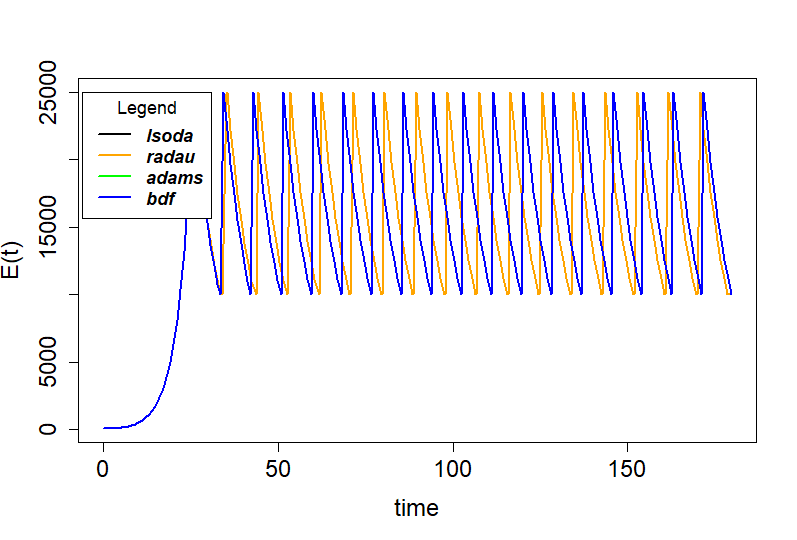
\includegraphics[width=0.7\linewidth]{./figures/solve_state_discontinuity_R}
\caption{Solving the state dependent discontinuity model in R}
\label{fig:solve_state_discontinuity_R}
\end{figure}
Several of the solvers in R have event detection capabilities. These are: `adams', `bdf', `lsoda', `Radau', and they will be used in this section to solve the state dependent discontinuity model using the approach described in the previous subsection. From Figure $\ref{fig:solve_state_discontinuity_R}$, we can see that all the solvers give solutions that are in agreement except `Radau'. This is in contrast with what happened previously when we were integrating a discontinuous problem, even at sharp tolerances. 

The case of `Radau' is interesting as it was giving a poor quality solution at the default tolerances, without event detection but it is now giving at least a solution that is exhibiting a correct pattern. We note that at sharp tolerances `Radau' with event detection gives results that approach the results from the other solvers, as shown in Figure $\ref{fig:solve_state_discontinuity_sharp_R}$. We will also note the poor performance of Radau in Table $\ref{tab:state_discontinuity_R}$. We also note that `Radau' Fortran code does not have built-in detection and that the event detection has been added through the C interface, which may explain the disparity in performance that we see for that solver.

\begin{figure}[H]
\centering
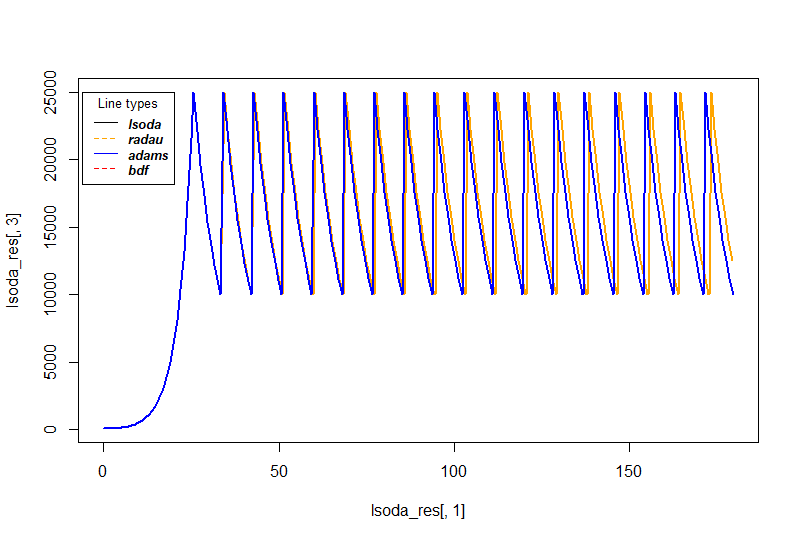
\includegraphics[width=0.7\linewidth]{./figures/solve_state_discontinuity_sharp_R}
\caption{Solving the state dependent discontinuity model in R at a sharp tolerance}
\label{fig:solve_state_discontinuity_sharp_R}
\end{figure}

We will show in Table $\ref{tab:state_discontinuity_R}$ that introducing event detection also makes the computation significantly more efficient while giving us more accurate results.

We note that it is unfair to compare the efficiency of the solvers at the default tolerances with the efficiency of the solvers when they use event detection as the results for the former are inaccurate.

\begin{table}[h]
\caption {Efficiency data for R state-dependent discontinuity model - number of function evaluations} 
\label{tab:state_discontinuity_R}
\begin{center}
\begin{tabular}{ c c c c c } 
method & no event & no event-sharp tol. & with event & with event-sharp tol.\\ 
lsoda & 2135 & 4658 & 1248 & 3435 \\
radau & 1002 & 21835 & 2151 & 14681\\
bdf & 3300 & 9803 & 1678 & 7963\\
adams & 1368 & 3467 & 817 & 2689\\
\end{tabular}
\end{center}
\end{table}

We can see from Table $\ref{tab:state_discontinuity_R}$ that with event detection we are gaining an improvement of around 1000 function evaluations for `lsoda', 7000 in `Radau' (sharp tol comparison), 2000 in `bdf', and 500 in `adams' while having more accuracy. This significant decrease in the number of function evaluations will lead to much faster CPU times, especially when the right-hand side function, $f(t, y)$ is more complex.

Also, we can see from the table that the solvers use fewer function evaluations compared with event detection than without event detection at the default tolerances. When comparing the values at the sharp tolerances, the use of event detection also decreased the respective number of function evaluations.

We also note that the Fortran code for `Radau' does not have event detection and that event detection was added through the R interface.

\subsubsection{Solving the state-dependent discontinuity model in Python using event detection}
\begin{figure}[H]
\centering
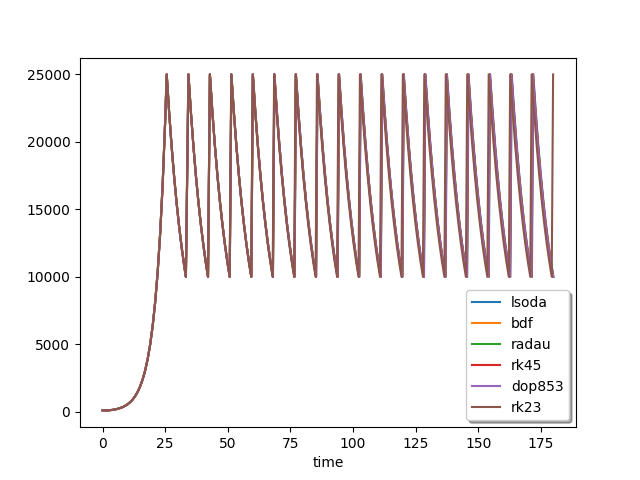
\includegraphics[width=0.7\linewidth]{./figures/solve_state_discontinuity_py}
\caption{Solving the state dependent discontinuity model in Python}
\label{fig:solve_state_discontinuity_py}
\end{figure}
All the solvers in Python have event detection and thus all will be used in this part of the study. In Python, $solve\_ivp()$ does not stop when an event is detected by default. We thus need to set the terminal flag of the root functions.
(Example: $root\_10000.terminal = True$).
Again, Figure $\ref{fig:solve_state_discontinuity_py}$ shows that all the solvers give solutions that are in agreement, suggesting that this is the correct solution. This is different from our results at sharp tolerances when event detection was not employed. We will also see that this is a much more efficient approach across all the solvers. The $solve\_ivp()$ implementation of `Radau' is in Python itself and thus it is different from the R implementation. We note that we did not have to provide the Python `Radau' implementation with a sharp tolerance to make its performance align with the other solvers' performances, suggesting that the issue in R may be due to the C implementation of event detection.

As is the case with R, we cannot compare the default tolerance efficiency data to the event detection efficiency data as the former corresponds to inaccurate results. So, in Table $\ref{tab:state_discontinuity_Py}$, we compare the sharp tolerance efficiency data with the data from the event detection computation.

\begin{table}[h]
\caption {Efficiency data for Python state-dependent discontinuity model - number of function evaluations} \label{tab:state_discontinuity_Py}
\begin{center}
\begin{tabular}{ c c c c } 
method & no event & no event with sharp tol. & with event detection \\ 
lsoda & 2357 & 4282 & 535 \\
bdf & 2301 & 11794 & 808 \\
radau & 211 & 74723 & 990 \\
rk45 & 1484 & 17648 & 674 \\
dop853 & 11129 & 21131 & 1514 \\
rk23 & 4307 & 246644 & 589 \\
\end{tabular}
\end{center}
\end{table}

Table $\ref{tab:state_discontinuity_Py}$ shows that the number of function evaluations when the solvers use event detection is far less when they do not; `LSODA' used around 3000 fewer function evaluations, `BDF' used 11000 less, `Radau' used 74000 less, `RK45' used 17000 less, `DOP853' used 20000 less and `RK23' used 246000 less. The reduction in CPU times from this will be significant across all the solvers, especially with a more complex right-hand side function.

\subsubsection{Solving the state-dependent discontinuity model in Scilab using event detection}
\begin{figure}[H]
\centering
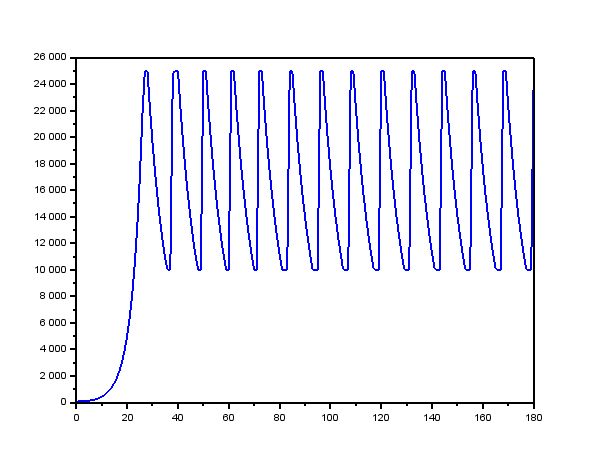
\includegraphics[width=0.7\linewidth]{./figures/solve_state_discontinuity_scilab}
\caption{Solving state discontinuity model in Scilab}
\label{fig:solve_state_discontinuity_scilab}
\end{figure}
There is only one solver with root functionality in Scilab; it is `lsodar', the root-finding version of `lsoda'. Judging from the solutions we obtained from Python and R, it seems that `lsodar' gives an accurate solution as well. It oscillates in the correct pattern and goes sharply between 10000 and 25000.

\begin{table}[h]
\caption {Efficiency data for Scilab state-dependent discontinuity model - number of function evaluations} \label{tab:state_discontinuity_scilab}
\begin{center}
\begin{tabular}{ c c c c } 
method & no event & no event with sharp tol. & with event detection \\ 
lsoda & 2794 & 4636 & 1327 \\
\end{tabular}
\end{center}
\end{table}

From Table $\ref{tab:state_discontinuity_scilab}$, we can see that the root-finding code uses fewer function evaluations that `lsoda' both at sharp and default tolerances.

\subsubsection{Solving the state-dependent discontinuity model in Matlab using event detection}
\begin{figure}[H]
\centering
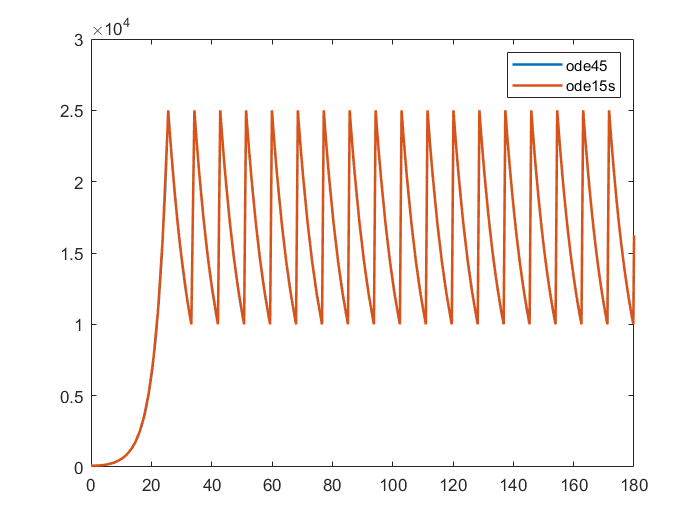
\includegraphics[width=0.7\linewidth]{./figures/solve_state_discontinuity_matlab}
\caption{Solving state discontinuity model in Matlab}
\label{fig:solve_state_discontinuity_matlab}
\end{figure}
Both $ode45$ and $ode15s$ have an event detection capability. (The root functions need to set an input parameter to indicate that the root is terminal in order to allow a cold start to be performed.) We applied event detection to solve the problem with the solvers in the Matlab environment and the results are shown in Figure $\ref{fig:solve_state_discontinuity_matlab}$. We remember that the solutions in Matlab without event detection were surprisingly accurate but were in disagreement with each other at points further in time. We can see that with event detection, the solutions are all in agreement at the default tolerances even at points further in time. We also see, in Table $\ref{tab:state_discontinuity_matlab}$, that the use of event detection is also more efficient than the computation without event detection.

\begin{table}[h]
\caption {Efficiency data for Matlab state-dependent discontinuity model - number of function evaluations} \label{tab:state_discontinuity_matlab}
\begin{center}
\begin{tabular}{ c c c c } 
method & no event & no event with sharp tol. & with event detection \\ 
ode45 & 2023 & 22411 & 859 \\
ode15s & 1397 & 11550 & 620 \\
\end{tabular}
\end{center}
\end{table}

We can see in Table $\ref{tab:state_discontinuity_matlab}$ that the computation with event detection uses fewer function evaluations than the code without event detection at default and sharp tolerances. We see that the computations with sharp tolerances, although they give acceptable solutions, use 20000 more function evaluations for $ode45$ than the computation with event detection and 11000 in the case of $ode15s$ than the computation with event detection.

\subsection{Efficiency data and tolerance study for the state dependent discontinuity problem}
\label{subsection:state_tolerance_study}
In this section, we will investigate how sharpening the tolerance improves the results in the case of the non-event detection experiment. We will also investigate coarsening the tolerance with event detection to show how coarse a tolerance we can use while getting acceptable results.

We will perform this analysis on LSODA across R, Python, and Scilab, as they appear to use the same source code, and with R and Python versions of DOPRI5 which do not use the same code but do use the same Runge-Kutta pair and with the Scilab version of RKF45 which is not the same code, nor the same pair but is a Runge-Kutta pair of the same order. We also use $ode45$ in Matlab as it is an implementation of DOPRI5 in Matlab. 

\subsubsection{Comparing LSODA across platforms for the state discontinuous problem}
\subparagraph{State dependent discontinuity LSODA tolerance study in R}
In this section, we use the R version of LSODA at multiple tolerances. We set both the relative and the absolute tolerance to various values and examine the solutions.

\begin{figure}[h]
\centering
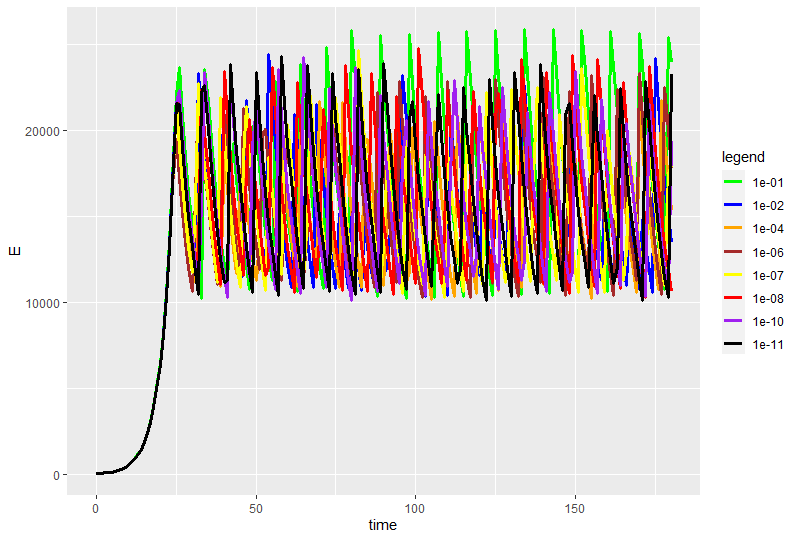
\includegraphics[width=0.7\linewidth]{./figures/tolerance_state_lsoda_no_event_R}
\caption{State dependent discontinuity model tolerance study on the R version of LSODA without event detection}
\label{fig:tolerance_state_lsoda_no_event_R}
\end{figure}

\begin{figure}[h]
\centering
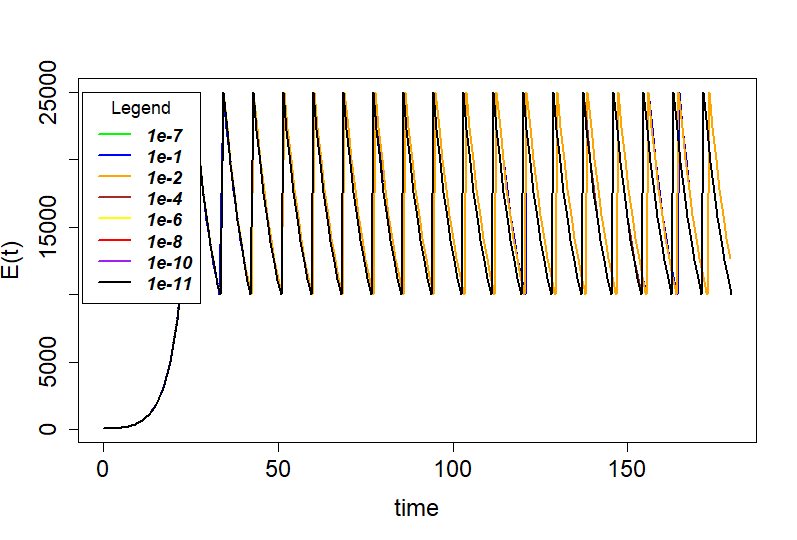
\includegraphics[width=0.7\linewidth]{./figures/tolerance_state_lsoda_with_event_R}
\caption{State dependent discontinuity model tolerance study on the R version of LSODA with event detection}
\label{fig:tolerance_state_lsoda_with_event_R}
\end{figure}

Figure $\ref{fig:tolerance_state_lsoda_no_event_R}$ shows that LSODA without event detection applied to the same problem at different tolerances gives vastly different results. We would expect the solutions at the sharper tolerances to be along very similar curves but that is not the case. This further supports our statement that for any state-dependent discontinuity, we cannot get reasonable results simply by sharpening the tolerance.

From Figure $\ref{fig:tolerance_state_lsoda_with_event_R}$, we can see the clear advantage of using event detection. Event detection allows us to use tolerances of $10^{-3}$ and sharper to get reasonable results while the computation without event detection failed even at a tolerance of $10^{-13}$. We also analyze the differences in efficiency between the two modes of operation of LSODA in Table $\ref{tab:tolerance_state_discontinuity_lsoda_R}$.

\begin{table}[h]
\caption {The R version of LSODA applied to state-dependent discontinuity model tolerance study - number of function evaluations} \label{tab:tolerance_state_discontinuity_lsoda_R} 
\begin{center}
\begin{tabular}{ c c c }
tolerance & no event detection & with event detection \\
1e-01 & 675 & 560 \\
1e-02 & 1856 & 522 \\
1e-04 & 1863 & 752 \\
1e-06 & 2135 & 1248 \\
1e-07 & 2676 & 1874 \\
1e-08 & 2730 & 2060 \\
1e-10 & 3337 & 2604 \\
1e-11 & 3603 & 3054 \\
\end{tabular}
\end{center}
\end{table}

Table $\ref{tab:tolerance_state_discontinuity_lsoda_R}$ shows a decrease in the number of function evaluations when event detection is employed across all tolerances which will translate into faster CPU times when the right-hand side function is more complex. We note that the comparison is unfair as the computations without event detection do not give a reasonably accurate answer. Furthermore, the latter computations use more function evaluations. This supports our conclusion that event detection is the appropriate way to solve state-dependent discontinuity problems when the discontinuity can be characterized in terms of an event.

\subparagraph{State dependent discontinuity model LSODA tolerance study in Python}
In this section, we use the Python version of LSODA at multiple tolerances to see how it performs. We recall that LSODA without event detection, even at very sharp tolerances, in Python was still not giving accurate results but we will see how the solutions change as the tolerance is sharpened. We will also show that coarse tolerances can be used with the computation that uses event detection. 

\begin{figure}[h]
\centering
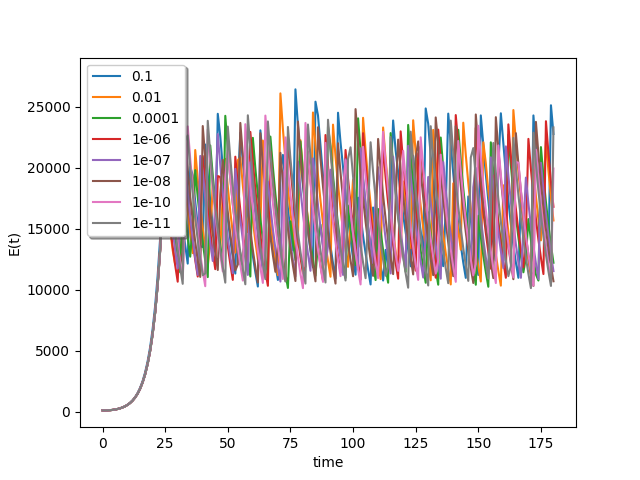
\includegraphics[width=0.7\linewidth]{./figures/tolerance_state_lsoda_no_event_py}
\caption{State dependent discontinuity model tolerance study on the Python version of LSODA without event detection}
\label{fig:tolerance_state_lsoda_no_event_py}
\end{figure}

\begin{figure}[h]
\centering
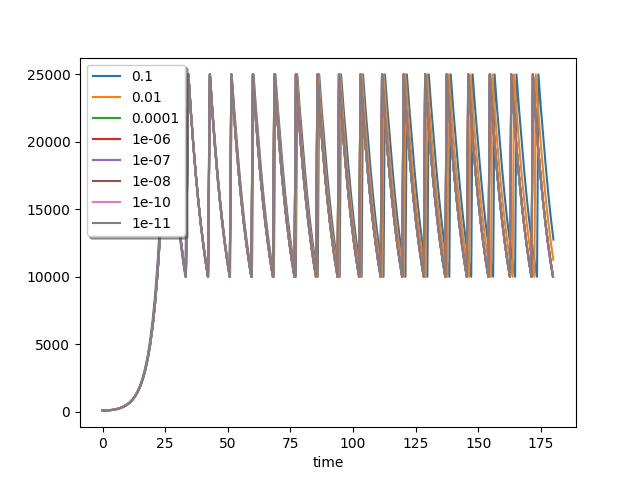
\includegraphics[width=0.7\linewidth]{./figures/tolerance_state_lsoda_with_event_py}
\caption{State dependent discontinuity model tolerance study on the Python version of LSODA with event detection}
\label{fig:tolerance_state_lsoda_with_event_py}
\end{figure}

Again Figure $\ref{fig:tolerance_state_lsoda_no_event_py}$ exposes that LSODA applied to the same problem at different tolerances gives substantially different results. We would expect the computations at the sharper tolerances to give quite similar results but this is not the case.

From Figures $\ref{fig:tolerance_state_lsoda_with_event_py}$ and $\ref{fig:tolerance_state_lsoda_no_event_py}$, we can see that the addition of event detection allows for the use of a coarser tolerance. We also note that the computations with event detection blur as we go further in time. This is because the coarser tolerance computations are not giving a sufficiently accurate solution. In Python, it is at a tolerance of $10^{-4}$ and sharper that we get reasonably accurate results. 

We analyse the efficiency of the computations in Table $\ref{tab:tolerance_state_discontinuity_lsoda_py}$. We must note that this analysis is unfair as the computation without event detection does not give an accurate solution to the problem. Still, we will see that the event detection computation uses fewer function evaluations while getting a more accurate answer.

\begin{table}[h]
\caption {The Python version of LSODA applied to state-dependent discontinuity model tolerance study - number of function evaluations} \label{tab:tolerance_state_discontinuity_lsoda_py} 
\begin{center}
\begin{tabular}{ c c c }
tolerance & no event detection & with event detection \\
0.1 & 1207 & 425 \\
0.01 & 1627 & 454 \\
0.0001 & 1968 & 689 \\
1e-06 & 2122 & 1305 \\
1e-07 & 2684 & 1807 \\
1e-08 & 2730 & 2099 \\
1e-10 & 3337 & 2639 \\
1e-11 & 3603 & 3098 \\
\end{tabular}
\end{center}
\end{table}

\subparagraph{State dependent discontinuity model LSODA tolerance study in Scilab}

We perform the same experiment in Scilab. We set the absolute and relative tolerance to the same values as in the other experiments and run the solvers. For the different tolerance values, we plot the solutions and examine how the solutions computed without event detection change as the tolerance is sharpened; we also examine how coarse a tolerance we can use with the event detection solver.

\begin{figure}[h]
\centering
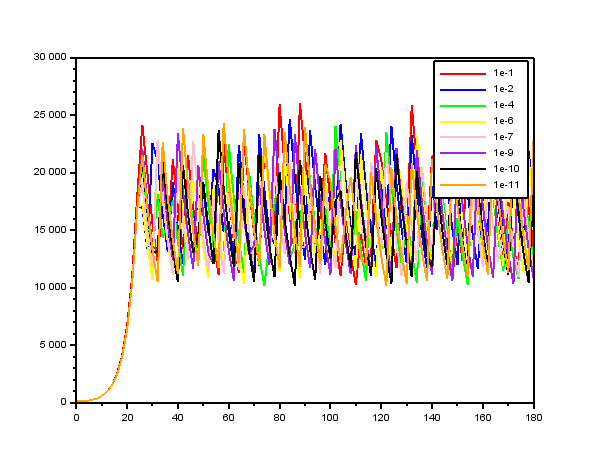
\includegraphics[width=0.7\linewidth]{./figures/tolerance_state_lsoda_no_event_sci}
\caption{State dependent discontinuity model tolerance study on the Scilab version of LSODA without event detection}
\label{fig:tolerance_state_lsoda_no_event_sci}
\end{figure}

\begin{figure}[h]
\centering
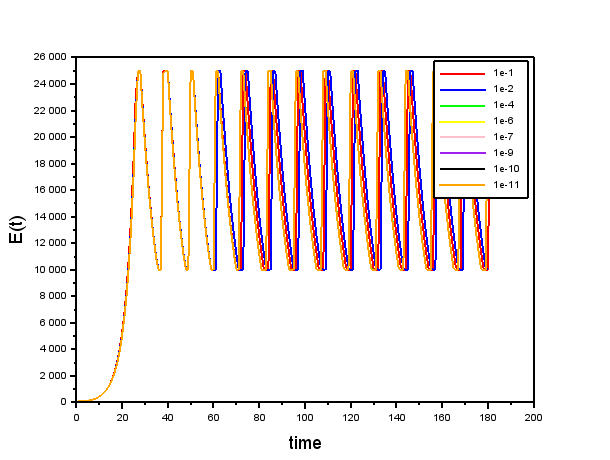
\includegraphics[width=0.7\linewidth]{./figures/tolerance_state_lsoda_with_event_sci}
\caption{State dependent discontinuity model tolerance study on the Scilab version of LSODA with event detection}
\label{fig:tolerance_state_lsoda_with_event_sci}
\end{figure}

Again, Figure $\ref{fig:tolerance_state_lsoda_no_event_sci}$ exposes the behavior whereby the same solver applied to the same problem at different tolerances gives substantially different results. We would expect the code at the sharper tolerances to give very similar curves but clearly, LSODA, even at sharp tolerances, does not.

From Figure $\ref{fig:tolerance_state_lsoda_with_event_sci}$, we can see that the use of the event detection allows us to use a coarser tolerance. We can use a tolerance of $10^{-3}$ and still get an accurate answer whereas, without event detection, even a tolerance of $10^{-12}$ is not sufficient.

\begin{table}[h]
\caption {The Scilab version of LSODA applied to state-dependent discontinuity model tolerance study - number of function evaluations} \label{tab:tolerance_state_discontinuity_lsoda_scilab} 
\begin{center}
\begin{tabular}{ c c c }
tolerance & no event detection & with event detection \\
0.1 & 1141 & 287 \\
0.01 & 1606 & 262 \\
0.0001 & 1968 & 523 \\
0.000001 & 2122 & 983 \\
0.0000001 & 2684 & 1307 \\
1.000D-08 & 2730 & 1567 \\
1.000D-10 & 3380 & 1963 \\
1.000D-11 & 3603 & 2331 \\
\end{tabular}
\end{center}
\end{table}

Table $\ref{tab:tolerance_state_discontinuity_lsoda_scilab}$ shows the number of function evaluations that LSODA uses with and without event detection to solve the state dependent discontinuity problem at multiple tolerances. We can see that even at coarse tolerances, using event detection allows LSODA use fewer function evaluations while giving more accurate solutions. This reinforces that event detection is the better way to solve state-dependent discontinuity problems. 

\subsubsection{Comparing Runge-Kutta pairs across platforms for state discontinuous problem}
In this section, we consider solvers based on Runge-Kutta pairs of the same order: DOPRI5 in R aliased as `ode45', DOPRI5 in Python aliased as `RK45', DOPRI5 in Matlab through the $ode45$ function, and RKF45 in Scilab aliased as `rkf'.

We recall that without event detection, none of these solvers across the platforms solved the problem to reasonable accuracy even with sharp tolerances. We will show what happens to these solvers as the tolerance is sharpened. We also coarsen the tolerance for the case where the solvers use event detection to see how coarse the tolerance can be while still obtaining reasonable accuracy.

\subparagraph{Tolerance study on state dependent discontinuity model using the R version of DOPRI5}
The R version of DOPRI5 does not have event detection but we still perform the experiment on this solver without event detection. We pick several values for the absolute and relative tolerances and run the solvers. In so doing we see how the code performs as the tolerance is sharpened. 

\begin{figure}[h]
\centering
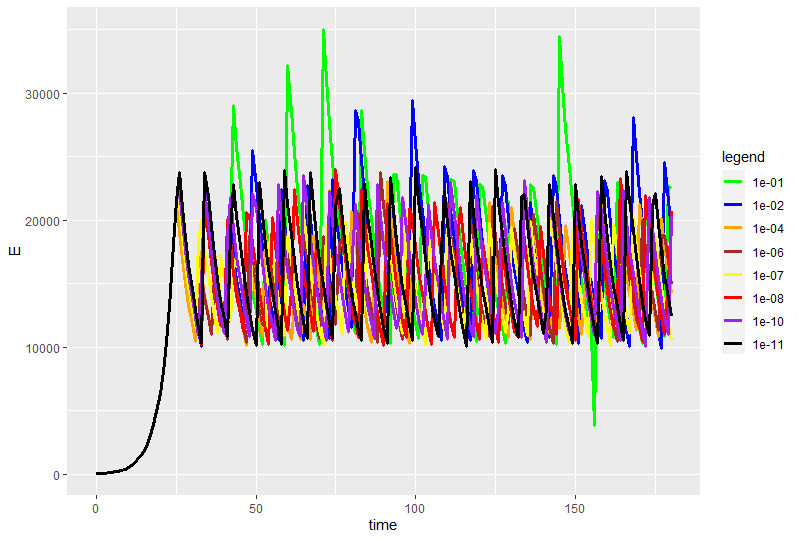
\includegraphics[width=0.7\linewidth]{./figures/tolerance_state_rk45_no_event_R}
\caption{State dependent discontinuity model tolerance study on the R version of DOPRI5 without event detection}
\label{fig:tolerance_state_rk45_no_event_R}
\end{figure}

From Figure $\ref{fig:tolerance_state_rk45_no_event_R}$, we see that DOPRI5 applied to the same problem with different tolerances, gives significantly different solutions. We then report the efficiency data for this case in Table $\ref{tab:tolerance_state_discontinuity_rk45_R}$. Table $\ref{tab:tolerance_state_discontinuity_rk45_R}$ shows the number of function evaluations the `ode45' solver uses. As it does not have event detection unlike the equivalent solvers in Python and Matlab, we cannot compare how the number of function evaluations differs with and without event detection. However, looking at the efficiency data of the Runge-Kutta pairs in the other environment and with R's LSODA solver, we can argue that it too will use less function evaluations with event detection than without.

\begin{table}[h]
\caption {The R version of DOPRI5 applied to state-dependent discontinuity model tolerance study - number of function evaluations} \label{tab:tolerance_state_discontinuity_rk45_R} 
\begin{center}
\begin{tabular}{ c c }
tolerance & no event detection \\
1e-01 & 1082 \\
1e-02 & 1142 \\
1e-04 & 2014 \\
1e-06 & 2027 \\
1e-07 & 2193 \\
1e-08 & 2919 \\
1e-10 & 5194 \\
1e-11 & 7690 \\
\end{tabular}
\end{center}
\end{table}

\subparagraph{Tolerance study on state dependent discontinuity model using the Python version of DOPRI5}
We perform the same experiment in Python. The Python version of DOPRI5 does have an event detection capability. The absolute and relative tolerances are set to a range of values and the solver is run both with and without event detection. We report on how the code performs as the tolerance is sharpened in the case without event detection. Since the Python version of DOPRI5 has event detection, we will see how coarse the tolerance can be set while still giving us a reasonably accurate solution. We will use results from the Runge-Kutta pair in Python and in Matlab, that both have event detection, to inform on how we can expect the results from the Scilab `rkf' and  the R `ode45' solvers, which do not have event detection, are supposed to be. We note that the solver crashes if we ask for a tolerance of 0.1.

\begin{figure}[h]
\centering
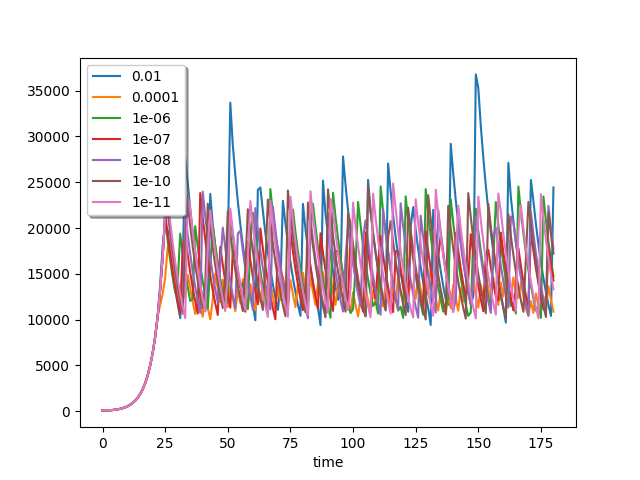
\includegraphics[width=0.7\linewidth]{./figures/tolerance_state_rk45_no_event_py}
\caption{State dependent discontinuity model tolerance study on the Python version of DOPRI5 without event detection}
\label{fig:tolerance_state_rk45_no_event_py}
\end{figure}

\begin{figure}[h]
\centering
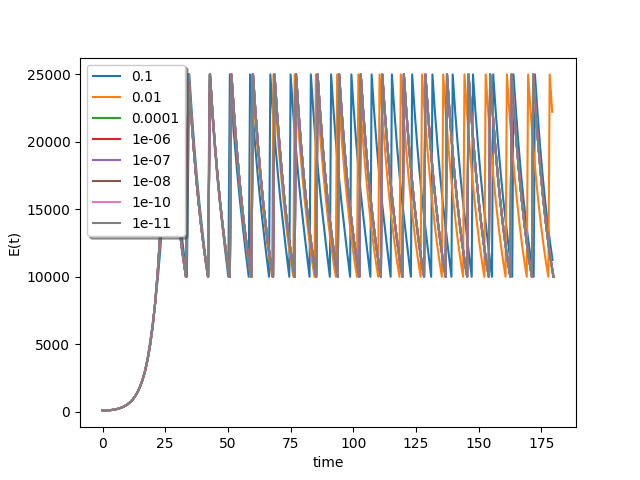
\includegraphics[width=0.7\linewidth]{./figures/tolerance_state_rk45_with_event_py}
\caption{State dependent discontinuity model tolerance study on the Python version of DOPRI5 with event detection}
\label{fig:tolerance_state_rk45_with_event_py}
\end{figure}

In Figure $\ref{fig:tolerance_state_rk45_no_event_py}$ corresponding to the case with no event detection, we can see that even at sharp tolerances, the solver is not able to compute a reasonably accurate solution. In contrast, in Figure $\ref{fig:tolerance_state_rk45_with_event_py}$, which corresponds to the case when we use event detection, the code can use very coarse tolerances. We can see that a tolerance of $10^{-4}$ is sharp enough to solve the given problem accurately; the blurring that occurs is due to the coarser tolerances. We present the efficiency data in Table $\ref{tab:tolerance_state_discontinuity_rk45_py}$ to show how the code with event detection is also far more efficient.

\begin{table}[h]
\caption {The Python version of DOPRI5 apllied to state-dependent discontinuity model tolerance study - number of function evaluations} \label{tab:tolerance_state_discontinuity_rk45_py} 
\begin{center}
\begin{tabular}{ c c c }
tolerance & no event detection & with event detection \\
0.01 & 1400.0 & 664.0 \\
0.0001 & 8462.0 & 806.0 \\
1e-06 & 6248.0 & 1232.0 \\
1e-07 & 6848.0 & 1754.0 \\
1e-08 & 7082.0 & 2354.0 \\
1e-10 & 10262.0 & 5066.0 \\
1e-11 & 13058.0 & 7688.0 \\
\end{tabular}
\end{center}
\end{table}

We can see in Table $\ref{tab:tolerance_state_discontinuity_rk45_py}$ that across all the different tolerances, the solver with event detection requires fewer function evaluations, around several thousand fewer for the sharper tolerances. 

\subparagraph{Tolerance study on state dependent discontinuity model using the Scilab version of RKF45}
Scilab uses RKF45 which is a different Runge-Kutta pair from what is used in DOPRI5 but the pairs have the same order. It does not have event detection but we can still perform the experiment on the solver without event detection. We pick several values for the absolute and relative tolerances and run the solver. In so doing we see how the solver performs as the tolerance is sharpened. 

The Scilab version of `rkf' can only integrate up to time 90 as it has a hard cap of 3000 derivative evaluations but this is enough to see that even at sharper tolerances, the solutions are not in agreement. Figure $\ref{fig:tolerance_state_rk45_no_event_sci}$ shows that the problem cannot be solved by simply using sharper tolerances. 
\begin{figure}[h]
\centering
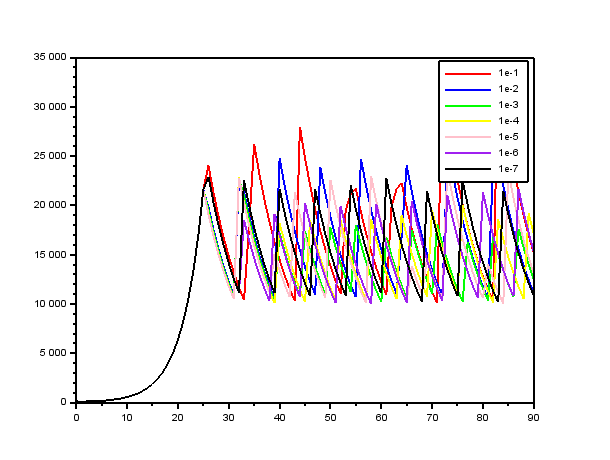
\includegraphics[width=0.7\linewidth]{./figures/tolerance_state_rk45_no_event_sci}
\caption{State dependent discontinuity model tolerance study on the Scilab version of RKF45 without event detection}
\label{fig:tolerance_state_rk45_no_event_sci}
\end{figure}

\begin{table}[h]
\caption {The Scilab version of RKF45 applied to state-dependent discontinuity model tolerance study - number of function evaluations} \label{tab:tolerance_state_discontinuity_rk45_scilab} 
\begin{center}
\begin{tabular}{ c c }
tolerance & no event detection \\ 
0.1 & 547 \\
0.01 & 732 \\
0.001 & 1294 \\
1e-4 & 1956 \\
1e-5 & 2364 \\
1e-6 & 2662 \\
1e-7 & 2802 \\
\end{tabular}
\end{center}
\end{table}

\subparagraph{Tolerance study on state dependent discontinuity model using the Matlab version of DOPRI5}
We apply different tolerances to the state problem with and without event detection the $ode45$ function which is a Matlab implementation of DOPRI5.

\begin{figure}[h]
\centering
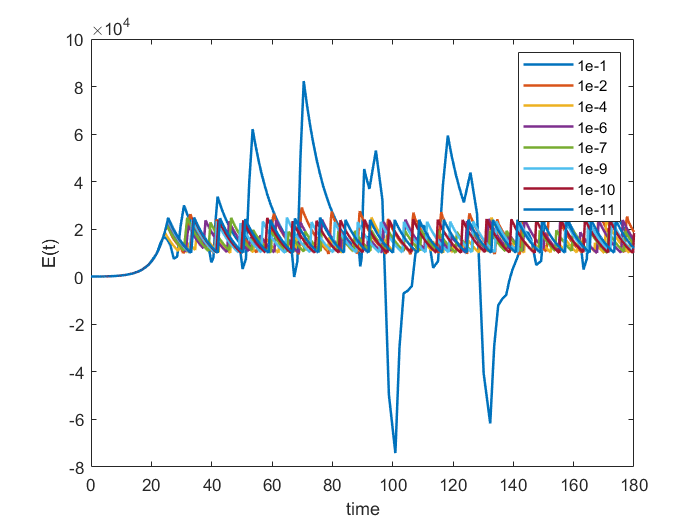
\includegraphics[width=0.7\linewidth]{./figures/tolerance_state_rk45_no_event_matlab}
\caption{State dependent discontinuity model tolerance study on the Matlab version of DOPRI5 without event detection}
\label{fig:tolerance_state_rk45_no_event_matlab}
\end{figure}

From Figure $\ref{fig:tolerance_state_rk45_no_event_matlab}$, we can see that the solution obtained with a tolerance of 0.1 is of poor quality without event detection. It does not follow the correct pattern of oscillating between 10000 and 25000. The computations of the other tolerances follow the correct pattern but are not in agreement.

\begin{figure}[h]
\centering
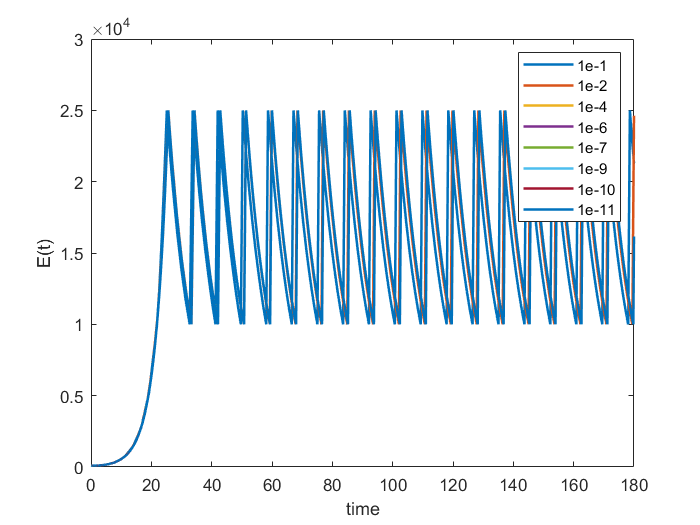
\includegraphics[width=0.7\linewidth]{./figures/tolerance_state_rk45_with_event_matlab}
\caption{State dependent discontinuity model tolerance study on the Matlab version of DOPRI5 with event detection}
\label{fig:tolerance_state_rk45_with_event_matlab}
\end{figure}
In Figure $\ref{fig:tolerance_state_rk45_with_event_matlab}$, we can see that the computations corresponding to most tolerances give solutions that are in agreement. A tolerance of 0.1 now follows the correct pattern but is not in agreement with the other tolerances at further points in time. For tolerances of $10^{-2}$ and sharper, we get accurate solutions.

\begin{table}[h]
\caption {The Matlab version of DOPRI5 applied to state-dependent discontinuity model tolerance study - number of function evaluations} 
\label{tab:tolerance_state_discontinuity_rk45_matlab} 
\begin{center}
\begin{tabular}{ c c c }
tolerance & no event detection & with event detection \\
0.1 & 415 & 650 \\
0.01 & 1339 & 661 \\
0.0001 & 4891 & 901 \\
1e-06 & 5803 & 1411 \\
1e-07 & 7225 & 1873 \\
1e-09 & 9739 & 4039 \\
1e-10 & 12385 & 6043 \\
1e-11 & 16357 & 9277 \\
\end{tabular}
\end{center}
\end{table}

Table $\ref{tab:tolerance_state_discontinuity_rk45_matlab}$, although being an unfair comparison since the solver without event detection did not give accurate solutions, shows that solving the problem without event detection is also less efficient. At the tolerance of 0.1, the smaller number of function evaluations for the solver without event detection is not relevant since the solution at a tolerance of 0.1 is very inaccurate. At all the other tolerances, the code with event detection is both more accurate and more efficient, usually using less than half the number of function evaluations.

